\section*{Q3: Temporal Difference}
\subsection*{1}

% TODO

\subsection*{2}

\begin{figure}[H]
    \centering
    \begin{subfigure}[b]{0.4\textwidth}
        \centering
        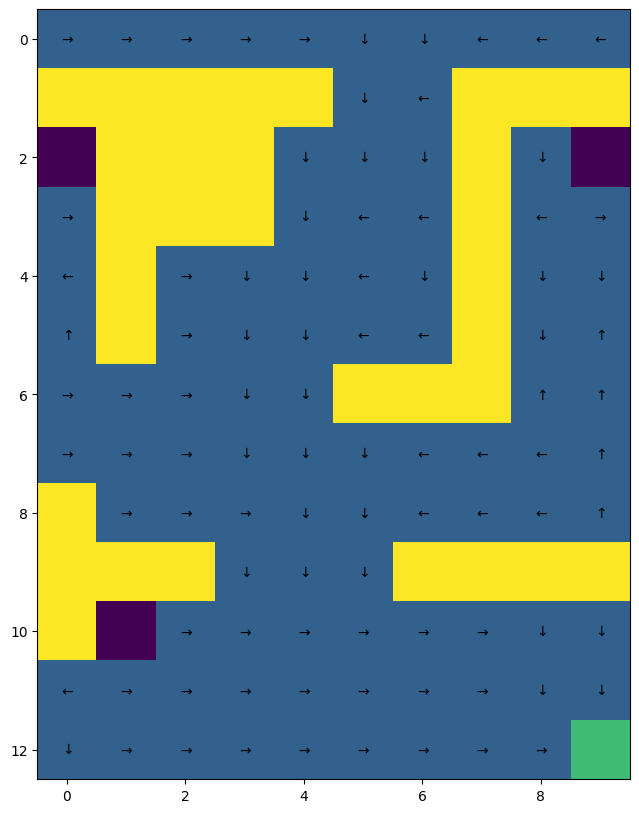
\includegraphics[width=\textwidth]{assets/td/td_policy.png}        
        \caption{Temporal Difference Policy}
    \end{subfigure}
    \hfill 
    \begin{subfigure}[b]{0.4\textwidth}
        \centering
        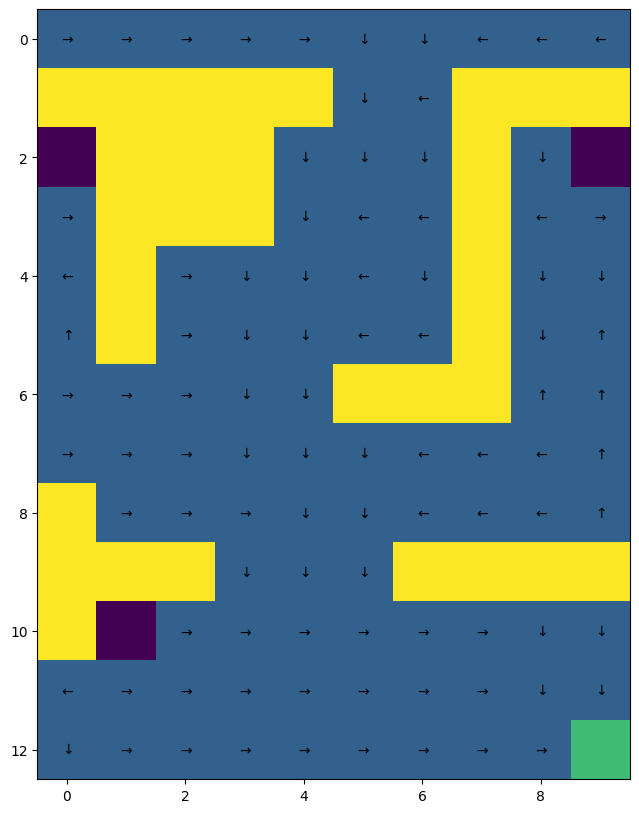
\includegraphics[width=\textwidth]{assets/td/td_policy.png}        
        \caption{Temporal Difference Value Function}
    \end{subfigure}
    \caption*{Graphical Representations of Temporal Difference Results}
\end{figure} 


\subsection*{3}

\begin{figure}[H]
    \centering
    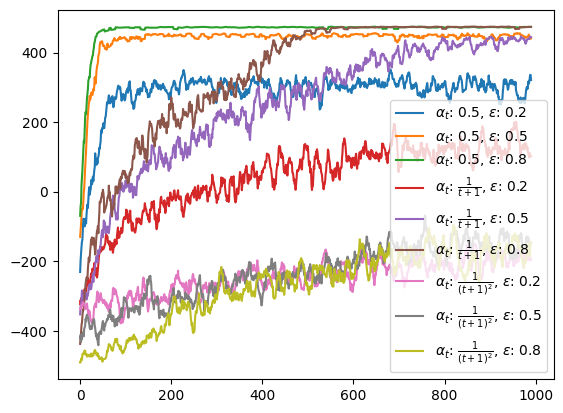
\includegraphics[width=\textwidth]{assets/td/td_analysis.png}        
    \caption{Temporal Difference analysis}
    \label{figure:temporal difference analysis}
\end{figure} 

In figure \ref{figure:temporal difference analysis}, the total reward
overtime is plotted for different configurations of the learning rate
(function for $\alpha_t$) and epsilon. The data smoothed out 
using a moving average make the data more legible.

It can be seen that having a high epsilon results in a faster 
convergence to the optimal policy. This is to be expected as 
low epsilon results in larger explorations of the environment,
whereas higher epsilon is more greedy - taking the current found 
optimal path more frequently. 